\chapter{Antecedentes y estado del arte} \label{chap:antecedentes}

En este capítulo se hará un repaso sobre los antecedentes y el estado del arte de la inteligencia artificial en la industria del videojuego, así como de las metaheurísticas y su uso en la investigación científica relacionada. Se usará la organización propuesta por Tommy Thompson en su artículo ``AI 101: How AI is Actually Used in the Video Games Industry'' \cite{thompson_how_2025}. Para guiar el proceso, se ha incluido la figura \ref{fig:ia_taxonomia} qué él desarrolló para su artículo, en la que se muestra un resumen de los usos a los que se les está dando a la IA en la industria del videojuego actualmente\footnote{Aunque no es un artículo científico, Tommy cuenta con más de 10 años de experiencia en la industria del videojuego, trabaja como consultor de IA para videojuegos y ha propulsado la creación del mayor congreso de IA en videojuegos de Europa. En la ``AI and Games Conference'' se reúnen profesionales de la industria y académicos para discutir sobre el estado del arte de la IA en videojuegos. Por lo tanto, su artículo se considera una buena referencia para entender cómo se está utilizando la IA actualmente en la industria del videojuego.}.

\begin{figure}
	\centering
	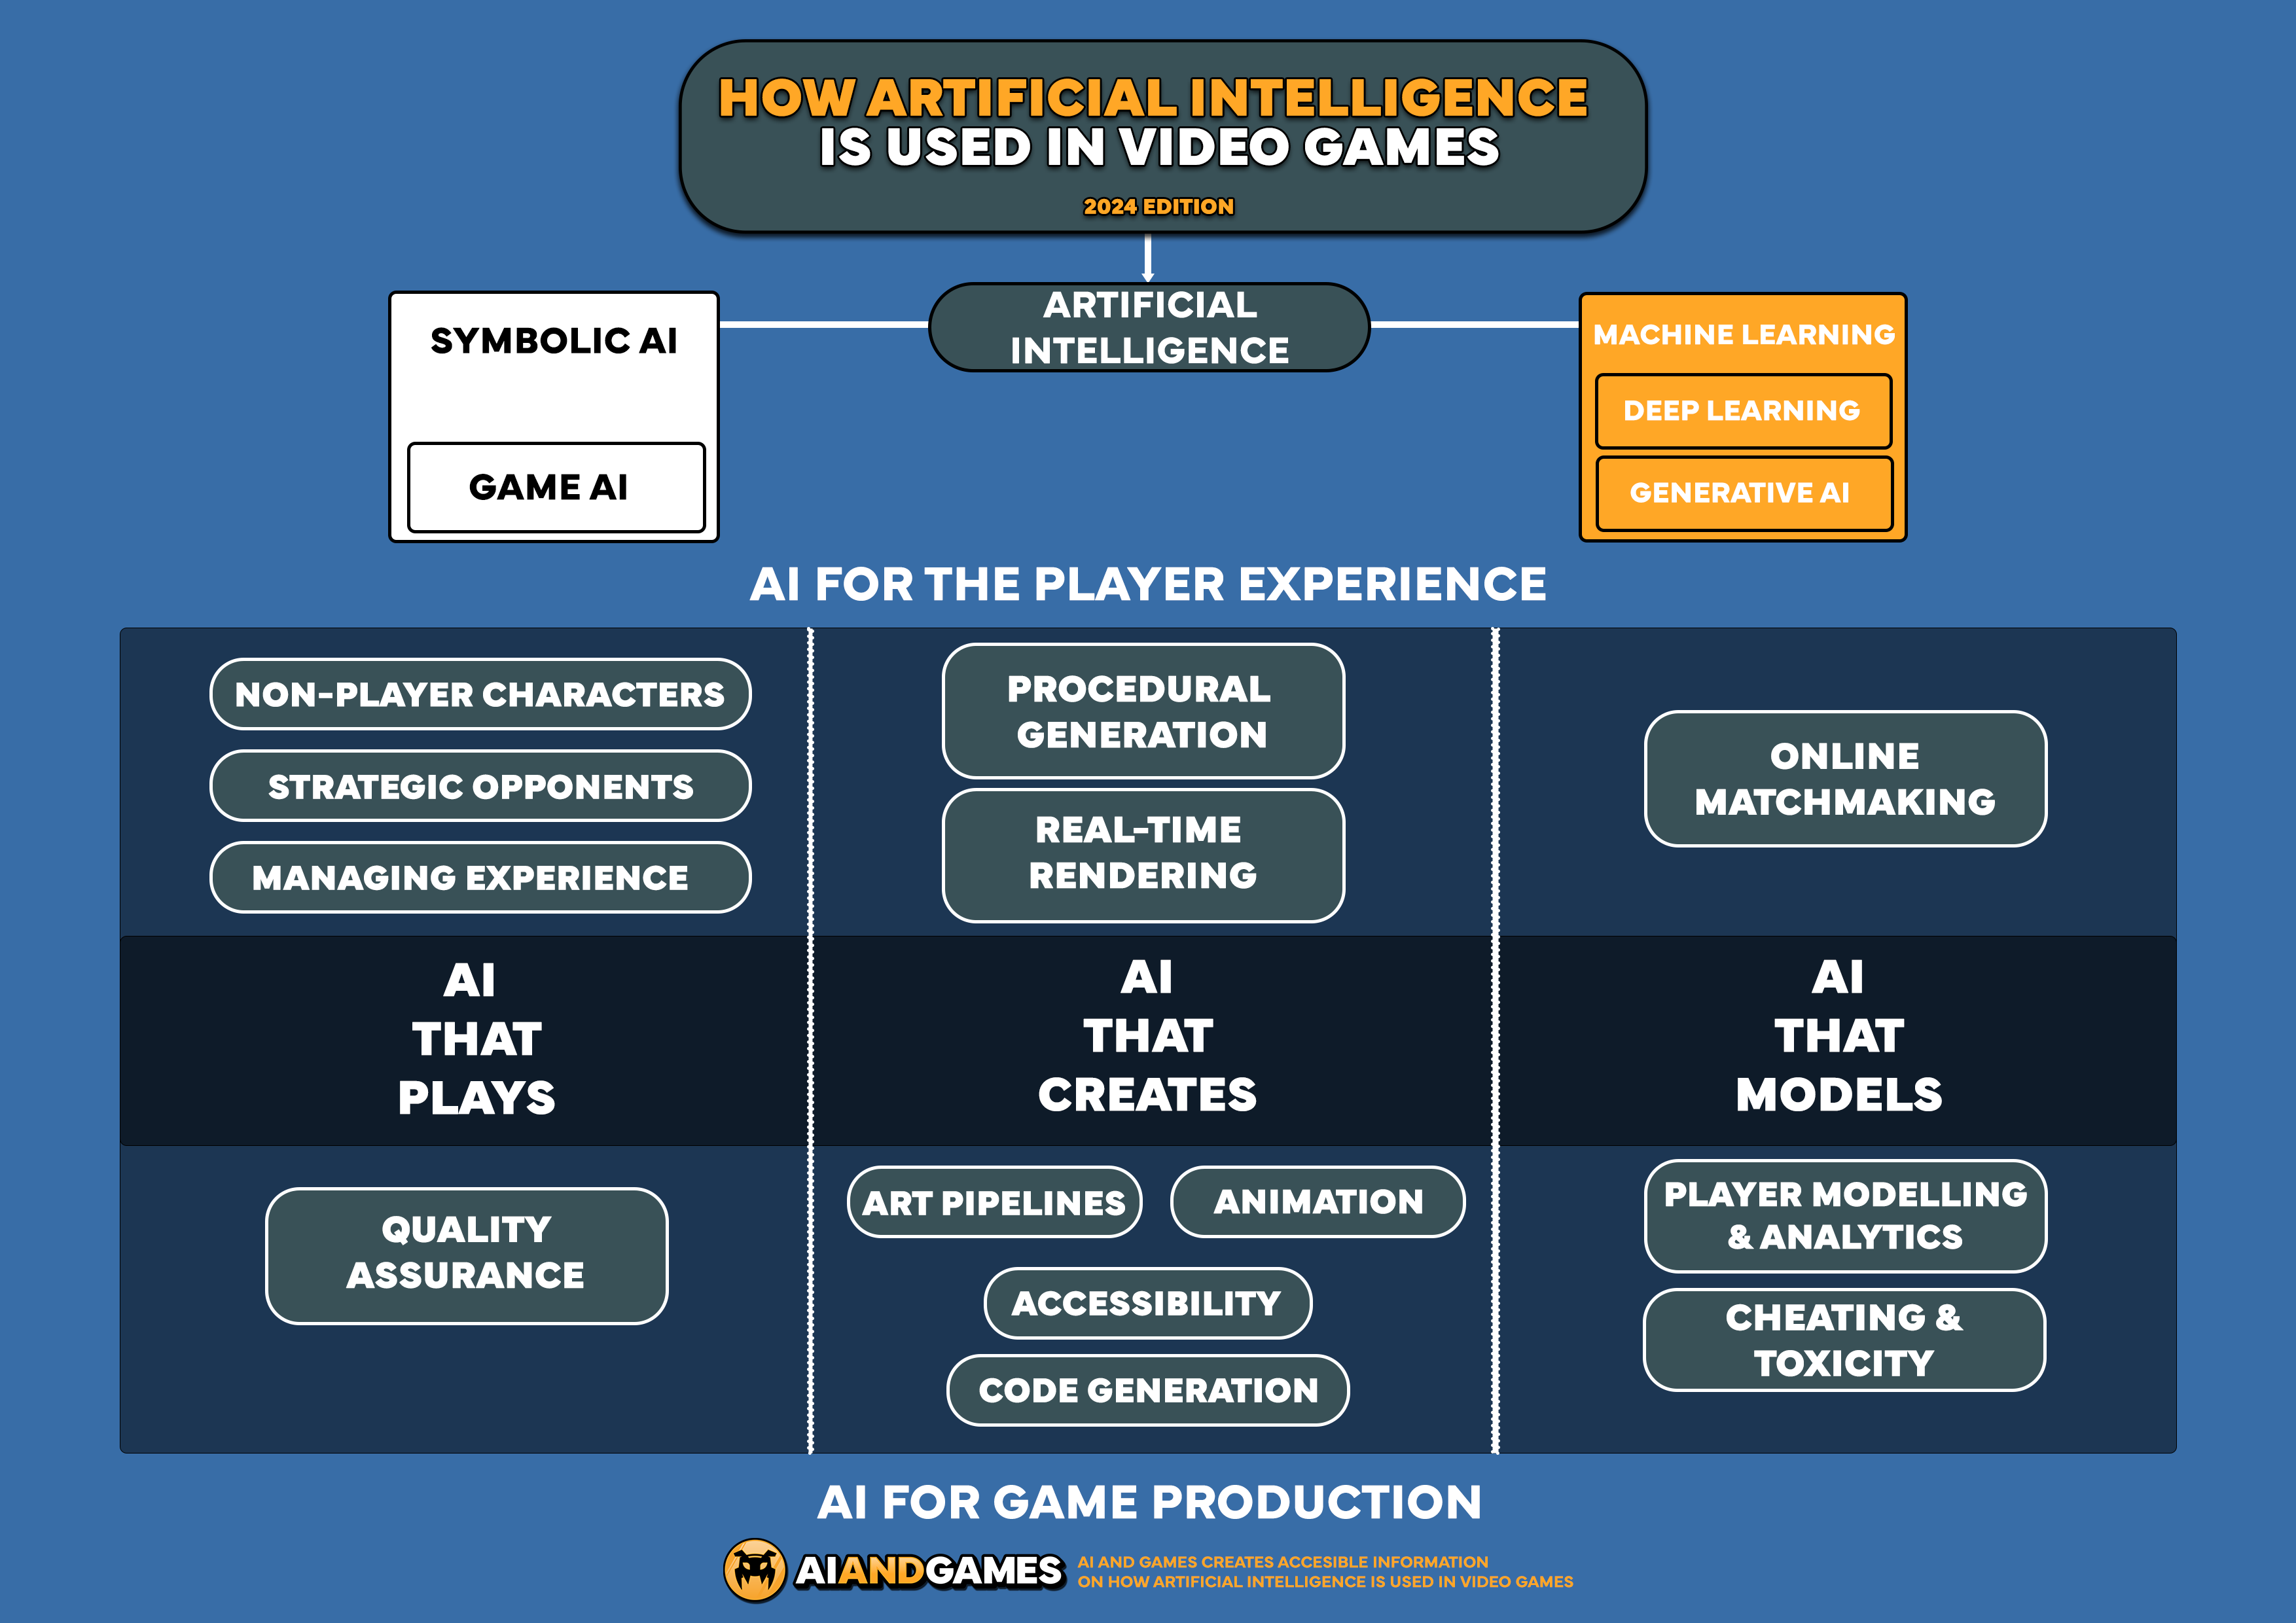
\includegraphics[width=1.0\textwidth]{img/AIforGames-Taxonomy.png}
	\caption{Taxonomía de la IA en videojuegos \cite{thompson_how_2025}.}
	\label{fig:ia_taxonomia}
\end{figure}

\section{Inteligencia artificial en videojuegos comerciales} \label{sec:ia_videojuegos}

Como ya se mencionaba en la introducción, la IA puede tener varias acepciones en función del contexto en el que se utilice. En el caso de los videojuegos, se pueden encontrar dos vertientes principales: la IA simbólica y el aprendizaje automático. La IA simbólica utiliza sistemas de razonamiento automático para modelar un problema y encontrar una solución dentro del espacio de búsqueda. Por otro lado, la IA basada en el aprendizaje automático utiliza métodos estadísticos que aprenden de datos existentes de diferentes formas, extendiéndose hasta el aprendizaje profundo y, de forma reciente, a la IA generativa. Este tipo de IA más avanzada, se está extendiendo rápidamente en la industria tecnológica, pero aún no se ha implementado de forma generalizada en el mundo del videojuego \cite{thompson_how_2025}.

Existe otra clasificación, la cual divide a la IA según su función dentro del videojuego. En este caso, se pueden distinguir tres tipos: la IA que juega al videojuego de alguna forma, la IA que crea partes del juego y la IA que modela una propiedad o fenómeno del ecosistema del videojuego. La primera categoría es la más relevante para este proyecto, pues se centra en la IA que controla a los personajes/enemigos o incluso la IA que pasa a ser un jugador virtual completo. Por esa razón, en este capítulo la mayoría de los ejemplos se centrarán en este tipo, aunque también se mencionarán algunos ejemplos de las otras categorías para dar una visión más completa al lector.

% En las siguientes subsecciones se realiza un breve repaso a las técnicas de inteligencia artificial más utilizadas a lo largo de la historia de los videojuegos, así como algunos ejemplos del estado del arte en el ámbito de la industria comercial del videojuego. Los usos de estos algoritmos no solo abarcan su función más habitual de enemigo o aliado, sino que también abarcan otros aspectos como la búsqueda de caminos o la deformación realista de las mallas \footnote{Una ``mesh'', o malla en español, es una estructura tridimensional formada por una colección de vértices, aristas y caras que definen la forma de un objeto 3D dentro de un videojuego \cite{universidad_europea_que_2025}.} de los personajes animados.

\subsection{Funciones hash}

Una de las técnicas más sencillas y antiguas para controlar partes específicas de un videojuego son las funciones hash. Este tipo de funciones simplemente reciben un conjunto de parámetros como entrada y devuelven un valor o acción a realizar. Dada su simplicidad, generan comportamientos predecibles, pero requieren de muy pocos recursos para su procesamiento y son fáciles de implementar. Un ejemplo clásico de IA basada en funciones hash es el en juego \textit{Space Invaders} \cite{wikipedia_artificial_2025} donde los invasores estaban controlados por este tipo de funciones.

\subsection{Máquinas de estados finitos}

Las máquinas de estados finitos son un modelo de computación conceptual que describe un sistema que solo puede encontrarse en un estado a la vez, y que puede cambiar a uno de sus otros estados como respuesta a ciertos eventos. Este mecanismo se ha utilizado y sigue utilizándose para un gran número de aplicaciones dentro de los videojuegos. Por ejemplo, en el juego \textit{Pac\-man}, la IA de los fantasmas se rije por el estado en el que se encuentran, como "cazando" o "siendo cazados" \cite{mike_game_2016}. Otro uso más centrado en la ``IA que crea'', está en la gestión de las animaciones de los personajes, donde cada estado corresponde a una posición o movimiento específico de la malla\footnote{Una ``mesh'', o malla en español, es una estructura tridimensional formada por una colección de vértices, aristas y caras que definen la forma de un objeto 3D dentro de un videojuego \cite{universidad_europea_que_2025}.}, que al mezclarse mediante interpolaciones generan animaciones. Al igual que las funciones hash, requieren de pocos recursos para su procesamiento, pero su naturaleza determinista y la posibilidad de entrar en bucles sin salida si no están bien diseñadas, limitan su uso en los escenarios más exigentes.

\subsection{Árboles de comportamiento}

Como evolución a las máquinas de estados finitos, surgieron los árboles de comportamiento, permitiendo un mayor grado de complejidad y flexibilidad en la toma de decisiones de los personajes. Los árboles de comportamiento son grafos dirijidos acíclicos, con nodos hoja que representan acciones y varios tipos de control de flujo que determinan el orden de ejecución de las hojas \cite{epic_games_behavior_2024}. Una de las características más útiles de los árboles de comportamiento es su modularidad, lo que permite reutilizar y combinar comportamientos específicos fácilmente. Un fantástico ejemplo de su correcto uso se expuso en la charla de la ``Game Developers Conference'' (GDC) de 2005, sobre la IA de \textit{Halo 2}, donde se explica que su capacidad de reutilización de árboles y el ser más sencillos de entender para los diseñadores del juego, hizo que los programadores optaran por su implementación en lugar de las máquinas de estados finitos \cite{isla_managing_2005}.


\subsection{Planificación de acciones orientada a objetivos y la IA utilitaria}

En contraste con los árboles de comportamiento, que generan una jerarquía de caminos, la planificación de acciones orientada a objetivos (GOAP, por sus siglas en inglés) es más parecida a la planificación de rutas, donde se busca el camino más óptimo para alcanzar un objetivo en función del estado del mundo. Cada uno de los pasos que llevan al objetivo tiene una serie de precondiciones que deben cumplirse, a los cuales se les puede asignar un coste. Es tal su similitud con la planificación de rutas, que este tipo de IA suelen utilizar internamente algoritmos de búsqueda como A*\footnote{El algoritmo A* también se utiliza para la búsqueda de caminos tradicional dentro de los videojuegos, es decir, para saber la ruta que debe tomar un objeto por el mapa para llegar a un destino.} para encontrar el camino más óptimo. Una de las mejores implementaciones de este tipo de IA se encuentra en el título de 2005 \textit{F.E.A.R.}, donde los enemigos y aliados utilizan GOAP para ``planificar'' su comportamiento una manera mucho más proactiva que sus predecesores \cite{jeff_gdc_2006}.

El caso de la IA utilitaria tiene un enfoque muy parecido, trata de ayudar a encontrar la mejor sucesión de acciones para alcanzar un objetivo, o incluso decidir cuál es el más adecuado en cada momento. Por ejemplo, un personaje que utilice IA utilitaria puede utilizar factores como la distancia a un objeto, el número de recursos existentes o el riesgo potencial de una acción para obtener una puntuación final que le permita decidir qué acción tomar. Esta forma de tomar decisiones contrasta con técnicas como los árboles de comportamiento, donde las acciones se ejecutan en un orden predefinido a menos que se produzca un cambio en el estado del mundo \cite{thompson_ai_2024}.

\subsection{Aprendizaje por refuerzo y redes neuronales}

El aprendizaje por refuerzo (RL, por sus siglas en inglés) es un subcampo del aprendizaje automático que trata de mejorar el comportamiento de un agente a través del feedback que recibe de su entorno. Utilizando un sistema de recompensas y penalizaciones, el agente aprende a tomar decisiones que maximicen su recompensa total a lo largo del tiempo. Aunque el RL empezó con técnicas tabulares, los algoritmos recientes incorporan redes neuronales en diferentes partes del proceso \cite{ghasemi_comprehensive_2025}. Quizás el ejemplo que más se suele ver en la literatura de videojuegos es el uso de RL para controlar vehículos autónomos. Una implementación de esta tecnología en un videojuego comercial está en el título \textit{Star Wars: Outlaws}, donde las motos controladas por IA utilizan un sistema de RL para moverse por el mapa o perseguir al jugador \cite{gaudreau_game_2025}. Sus desarrolladores argumentan que les permitió tener un sistema de control que se adapta a las diferentes rutas del juego sin importar los cambios en el mapa que haya entre versiones.

Pero el uso de redes neuronales no se limita a la toma de decisiones. Su capacidad para realizar inferencias rápidas a partir de datos complejos las hace ideales para otras tareas, como la deformación de mallas. El objetivo en este caso es evitar el fenómeno conocido como el ``valle inquietante'' (\textit{Uncanny Valley}), que se produce cuando una réplica de un ser humano es muy realista, pero no perfecta, generando una sensación de extrañeza en el espectador. Un personaje que sonríe, por ejemplo, pero cuyos músculos faciales alrededor de los ojos permanecen inmóviles, es un caso clásico de este efecto. Para intentar superar este problema, Epic Games optó por crear un sistema para Unreal Engine que utiliza modelos de redes neuronales que simulan el comportamiento de la musculatura y los tejidos blandos bajo la piel al extenderse y contraerse \cite{epic_games_ml_2025}. Un ejemplo de uso de esta reciente tecnología se puede encontrar en la demo técnica que CD Projekt Red mostró en el Unreal Fest de 2025 \cite{cd_projekt_red_witcher_2025}. En ella, se mostraba como se modelaba internamente la musculatura de un caballo para que sus animaciones de movimiento fueran mucho más realistas.

% Me parece que ya es suficiente con lo que hay. Quito esta sección y la siguiente.

% \subsection{Unión de varias técnicas}
% The Last of Us: Parte II --> muchos sistemas entrelazados
% Alien: Isolation --> Árbol de comportamiento + Director de IA

% \subsection{Modelos de IA generativa}
% No es una tecnología lo suficientemente madura como para uso actual en videojuegos comerciales.

\section{El problema de la IA en los videojuegos comerciales} \label{sec:problema_ia_videojuegos}

En la anterior sección se han hablado exclusivamente de técnicas de inteligencia artificial que se han empleado en videojuegos que han salido al mercado para el público general. Pero, salvo en funciones específicas como el movimiento de las motos en \textit{Star Wars: Outlaws}, no se ha mencionado el uso de técnicas de inteligencia artificial ``avanzadas'' para el control de los personajes o contrincantes virtuales. Sin embargo, este tipo de IAs sí existen. Se han desarrollado con éxito bots capaces de jugar a alto nivel videojuegos como \textit{StarCraft II} \cite{vinyals_grandmaster_2019}, \textit{Dota 2} \cite{openai_dota_2019} o \textit{Rocket League} \cite{moschopoulos_lucy-skg_2023}, entre otros. Todos estos artículos científicos, aclamados por la comunidad debido a su complejidad, tienen algo en común: se han creado una vez el juego ya había sido lanzado y era estable.

A menudo, los videojuegos con componentes multijugador de éxito, acaban siendo actualizados y mejorados durante años. Este clima de constance cambio, el cual se ve acentuado aun más durante la etapa inicial de su desarrollo, hace que el uso de técnicas como el aprendizaje por refuerzo, los algoritmo evolutivos o las redes neuronales sean especialmente difíciles de implementar. El ejemplo de \textit{Star Wars: Outlaws} es un caso muy reciente, con tecnología especialmente desarrollada para su motor gráfico y con un equipo detrás de cientos de personas con capacidad de delegar personal en enfoques más vanguardistas. Y aun así, sólo usaron el aprendizaje por refuerzo para un aspecto muy específico del videojuego. Se podría considerar un problema del tipo ``el huevo o la gallina'', pues se necesita que el juego esté prácticamente listo para entrenar al bot, lo que permite crear un bot específico para esa versión, pero si el juego cambia, incluso con pequeños ajustes de balanceo de poder, entonces el rendimiento del bot puede verse afectado. Por eso todos esos artículos científicos se centran en juegos ya terminados o en una versión específica del videojuego. En aquellos casos en los se ha conseguido crear un bot que maneje todos los aspectos del control, como lo fue para AlphaStar \cite{vinyals_grandmaster_2019} o OpenAI Five \cite{openai_dota_2019}, se han necesitado una gran cantidad de datos que solo se podrían haber obtenido gracias a la comunidad de jugadores de sus respectivos videojuegos y no antes de su lanzamiento.

Sin embargo, esto no significa que no se puedan crear ``IAs que juegan'' mediante aprendizaje automático para videojuegos aun en desarrollo. Simplemente se deben crear para resolver problemas específicos o bien para el caso de videojuegos que no requieran de un escenario tan complejo como los mencionados anteriormente \cite{ai_and_games_why_2024}. Un ejemplo de esto sería Sophy, la IA de conducción de \textit{Gran Turismo 7} \cite{wurman_outracing_2022}, que fue entrenada durante el desarrollo del videojuego para manejar los vehículos del videojuego de carreras.

A día de hoy es posible que esa sea la forma más adecuada de utilizar este tipo de técnicas: o bien para pequeñas características del juego, o bien para entornos más reducidos, como el caso de los videojuegos de cartas. En ese tipo de videojuegos, aunque el número de variables es alto, la cantidad de acciones posibles en cada turno es limitada, lo que permite entrenar a los bots de forma más eficiente. En las siguientes secciones se revisarán algunas de las investigaciones científicas que intentan aplicar este mismo enfoque a sus implementaciones.

\section{Metaheurísticas en la investigación científica sobre videojuegos} \label{sec:estado_arte}

% Papers extra que no se han incluido:
% ------------------------------------------------------------------------------------------------

% Procedural Generation of Quests for Games Using Genetic Algorithms and Automated Planning --> https://www.icad.puc-rio.br/~logtell/papers/Edirlei_SBGames_2019.pdf
% Evaluating Alternative Metaheuristic Algorithms for Procedural Content Generation in Game Design --> https://www.researchgate.net/publication/389270827_Evaluating_Alternative_Metaheuristic_Algorithms_for_Procedural_Content_Generation_in_Game_Design
% Systematic Literature Review of Meta-heuristic Algorithms and their Application in Procedural Content Generation (PCG) in the Context of Computer Games --> https://labs.sciety.org/articles/by?article_doi=10.21203/rs.3.rs-4883187/v1
% Procedural Video Game Scene Generation by Genetic and Neutrosophic WASPAS Algorithms: https://www.mdpi.com/2076-3417/12/2/772
% Comparative Analysis of Metaheuristic Algorithms for Procedural Race Track Generation in Games --> https://www.igi-global.com/article/comparative-analysis-of-metaheuristic-algorithms-for-procedural-race-track-generation-in-games/350330

% Continuous Spatial Public Goods Game Based on Particle Swarm Optimization with Memory Stability --> https://www.mdpi.com/2227-7390/10/23/4572

% AntBot: ant colonies for video games --> https://www.computer.org/csdl/journal/ci/2012/04/06262464/13rRUzpzeDF

% Evolutionary Artificial Intelligence for MOBA / Action-RTS Games using Genetic Algorithms --> https://www.ijcaonline.org/proceedings/icrtitcs2012/number10/10320-1465/#:~:text=The%20Genetic%20Algorithms%20hence%20defines,reactive%20response%20of%20the%20enemy.

% ------------------------------------------------------------------------------------------------

Las ``IAs que crean'' son una forma de llamar a aquellas aplicaciones de la inteligencia artificial que se centran en la generación procedural de contenido, la cual trata de unir y entremezclar diferentes bloques de construcción prehechos para crear nuevos elementos dentro del videojuego. Por ejemplo, se podrían utilizar varias texturas de manchas, ruido, metales y óxido para crear una única textura que muestre un material deteriorado por el tiempo, pero que tenga un aspecto único cada vez que se use. Otro ejemplo sería el de colocar diferentes plantas, rocas y árboles sobre un terreno para crear un bosque, pero siguiendo una serie de heurísticas (IA simbólica) para que el resultado sea creíble. Ya en 2011, Togelius et al. \cite{togelius_search-based_2011} publicaron una review sobre los diferentes enfoques que se estaban utilizando para la generación procedural de contenido en videojuegos, y cómo las metaheurísticas estaban siendo utilizadas para este fin. Uno de ellos era el sistema ``Ludi'', que codificaba las reglas del juego como árboles de expresión y usaba programación genética para generar conjuntos de reglas balanceadas para el videojuego. En su artículo, los autores dicen los sistemas existentes hasta la fecha, los cuales usaban enfoques basados en la simulación de procesos naturales, debían mejorar la consistencia, la rapidez y la personalización para el usuario si se quisieran utilizar en videojuegos comerciales a gran escala. 

Otro ejemplo de uso de metaheurísticas en la generación procedural de contenido es el trabajo de Geijtenbeek et al. \cite{geijtenbeek_flexible_2013} en 2013, donde se presenta un sistema de locomoción para criaturas bípedas que utiliza un algoritmo evolutivo para optimizar los pesos de las articulaciones necesarios para que la criatura se mueva adecuadamente. En su artículo, los autores muestran como los controladores eran capaces de adaptarse a diferentes terrenos con desnivel e incluso perturbaciones externas.

Más recientemente, en 2021, Snell et al. \cite{snell_evolutionary_2021} presentaron un enfoque evolutivo para el balanceo de videojuegos de estrategia en tiempo real. En su estudio, utilizaron diferentes variables dentro del videojuego para conseguir variaciones en la dificultad de un nivel sin desviarse demasiado de la experiencia original del mismo. Concluyeron que su enfoque era capaz de generar niveles similares, pero que se sentían diferentes, lo que permitía al jugador disfrutar de una experiencia más variada sin ser injusta.

\section{Algoritmos evolutivos en juegos de estrategia por turnos} \label{sec:trabajos_relacionados}

El bot presentado en este proyecto utiliza como base el trabajo de Ematerasu et al. \cite{ematerasu_scriptsoftribute_2022}, quienes desarrollaron el motor Scripts of Tribute (SoT) para el videojuego de cartas \textit{Tales of Tribute} de la saga \textit{The Elder Scrolls}. Pero este no es el único ni el primer motor capaz de simular partidas de juegos de cartas. Ya en 2002, MagiSoft desarrolló el software \textit{Magic Workstation} \cite{magi-soft_development_magic_2002}, que no solo se usó para jugar partidas online y que los jugadores pudieran enfrentarse entre ellos, sino también permitía construir sus propios mazos a los usuarios, que luego podrían usar en las partidas. Magic Workstation funcionaba con un gran número de juegos de cartas, como \textit{Magic: The Gathering} o \textit{Yu-Gi-Oh!}, pero hubo un juego que salió a la venta en 2014 y que estaba pensado desde el principio para ser jugado en línea: \textit{Hearthstone}. Este videojuego de cartas se convirtió rápidamente en uno de los más populares del mundo, y su comunidad de jugadores creció exponencialmente. Sin embargo, aunque ya era un entorno virtual de salida, no existía un software específico para crear y probar bots. En 2017, el equipo de HearthSim lanzó \textit{Sabberstone} \cite{hearthsim_hearthsimsabberstone_2017}, un motor de simulación que permitía hacer precisamente eso.

Pero no solo existen simuladores de juegos de cartas, un ejemplo de un motor que se adentra en un género relacionado, pero diferente, es \textit{Video Game Championships (VGC)}, un simulador de videojuegos de \textit{Pokémon} desarrollado por Reis et al. \cite{simao_reis_vgc_2019} en 2019. Este motor permite hacer lo propio con los combates \textit{Pokémon}, que aunque no son juegos de cartas, sí que utilizan un sistema de combate por turnos y una gran cantidad de variables a tener en cuenta.

% Paper de Pablo y TFG de los ganadores de la competición de IA de Tales of Tribute. Comparar sus enfoques al mio

\subsection{Optimización de agentes de Hearthstone mediante un algoritmo evolutivo}
% Pablo --> garcia-sanchez_optimizing_2020

El trabajo que ha servido como punto de partida para el desarrollo del bot de este proyecto es el de García-Sánchez et al. \cite{garcia-sanchez_optimizing_2020}, el director de este Trabajo de Fin de Máster. En su artículo, los autores utilizan un algoritmo evolutivo para optimizar el comportamiento de un bot en el motor de simulación de \textit{Sabberstone}. Primero, utilizaron el conocimiento experto para definir la lista de pesos que el bot utilizaría para generar la evaluación de cada jugada. Este enfoque centrado en datos de conocimiento prexistentes se mantiene en el bot desarrollado en este proyecto, pero con la diferencia de que el autor de este TFM nunca había jugado a Tales of Tribute antes de empezar a desarrollar el bot, por lo que no tenía ningún conocimiento previo sobre el videojuego. De esta manera, una de las primeras diferencias entre ambos trabajos es que el bot de este proyecto se basa en un conocimiento previo más general sobre los juegos de cartas (principalmente conocer las reglas del videojuego), aportando heurísticas para casos muy concretos, mientras que el bot de García-Sánchez et al. utiliza los cimientos de un jugador con mucha experiencia en el videojuego de cartas \textit{Hearthstone}.

Sin embargo, aunque el diseño de los pesos es ligeramente diferente, el enfoque del algoritmo evolutivo es muy similar. En el caso del bot de Sabberstone, no se tenía acceso a bots prexistentes contra los que competir, por lo que los autores optaron por utilizar una estrategia de coevolución. Siguiendo este enfoque, la población de 10 bots se enfrentaba entre sí para decidir cuáles eran los mejores. Tras el torneo, los mejores bots se seleccionaban para crear una nueva generación de bots, que se enfrentaban entre sí de nuevo. Después de un número específico de generaciones, el bot con mejor rendimiento se seleccionaba como el ganador. Este enfoque de coevolución se ha mantenido en el bot desarrollado en este proyecto, pero se ha expandido gracias a la posibilidad de utilizar bots prexistentes en Scripts of Tribute. Como se explica de forma más detallada en la sección \ref{sec:mecanismos_evaluacion_fitness}, el proceso de evolución cuenta con tres modos de evaluación: el modo de coevolución, el modo fijo (contra otros bots) y el modo híbrido (una combinación de ambos). Además, se implementó un mecanismo del estilo ``salón de la fama'' para guardar los mejores bots de cada entrenamiento y utilizarlos en otros. Todo ello expandiendo el nivel de paralelismo del algoritmo evolutivo, utilizando un diccionario de información común y accesible por todos los procesos de forma concurrente.

Uno de los agentes generados por el algoritmo evolutivo de García-Sánchez et al. quedó segundo en la competición de IA de \textit{Sabberstone} de 2018, lo que demuestra la efectividad de su enfoque coevolutivo y conocimiento experto.

\subsection{Desarrollo de un agente para el concurso de IA Tales of Tribute}

Scripts of Tribute también se utiliza para realizar competiciones entre bots, donde los participantes envían uno o varios agentes para competir entre sí. Por el momento se han realizado dos competiciones, una en 2023 y otra en 2024. En ambas, el bot ganador fue desarrollado por Adam Ciężkowski y Artur Krzyżyński \cite{adam_ciezkowski_developing_2023}, quienes utilizaron un enfoque basado en Monte Carlo Tree Search (MCTS) junto con optimización de pesos mediante algoritmos evolutivos para la toma de decisiones de su bot. 

El algoritmo de optimización de búsqueda MCTS lleva años utilizándose en la creación de IA para videojuegos, especialmente en aquellos con un alto número de variables y acciones posibles. Ya en 2018, se utilizó para crear un bot capaz de jugar a \textit{Hearthstone} \cite{swiechowski_improving_2018}, mientras que un año antes, AlphaZero comparaba diferentes búsquedas realizadas con MCTS para elegir la mejor jugada en partidas de ajedrez \cite{silver_mastering_2017}.

En el caso del bot de Adam y Artur, utilizan MCTS para explorar el espacio de búsqueda en aquellas situaciones en las que explorarlo completamente sería inviable. De esta manera, genera un arbol parcial de acciones enfocándose en aquellas jugadas que tienen más probabilidades de ser las mejores según su función de evaluación. Es decir, para cada jugada, el bot simula varias partidas futuras a partir de esa jugada de forma paralela, y en función del resultado de esas partidas, asigna un valor a la jugada. Dado que hay componentes de aleatoriedad en el videojuego, como el robo de cartas, cuantas más partidas simule, más preciso será el valor que le asigne a la jugada. Sin embargo, esto también significa que el tiempo de procesamiento del bot aumenta, por eso sus autores tuvieron que añadir un límite de tiempo para la generación del árbol. Además, para limitar el factor de ramificación del árbol, utilizaron diferentes heurísticas para descartar jugadas que no merecían la pena explorar, como el uso de aquellas cartas que siempre se deben jugar al principio del turno (lo que llamaron ``movimientos instantáneos'').

Como ya se ha mencionado, la función de evaluación del bot se basa en un conjunto de pesos que se usan para calcular el valor final de cada acción. Este enfoque es muy similar al utilizado por García-Sánchez et al. y por este mismo proyecto, pero con la diferencia de que sus autores no se enfocaron tanto en esta parte de su bot. Dado que su algoritmo ya necesitaba de una gran cantidad de código para implementar y optimizar MCTS, su función de evaluación tiene un número reducido de pesos (aproximadamente la mitad que en este trabajo), y no incorpora diferentes modos de ajuste de los pesos del algoritmo evolutivo, dejando de lado el enfoque coevolutivo y el híbrido. Aun así, su bot ha demostrado ser muy efectivo en las competiciones de IA de Scripts of Tribute, ganando ambas ediciones hasta la fecha (más información en la sección \ref{sec:competicion_ieee_cog}).

\todo{¿Con esto concluye el  OG7? Ver si puedo arreglar el MCTS para enfrentarlo a mi bot...}